% !TeX root = surprises.tex

\chapter{Cómo custodiar un museo}\label{c.museum}

%%%%%%%%%%%%%%%%%%%%%%%%%%%%%%%%%%%%%%%%%%%%%%%%%%%%%%%%%%%%%%%

En 1973 Victor Klee se preguntó cuántos custodios son necesarios para vigilar todas las paredes de un museo. Si las paredes forman un polígono regular o incluso un polígono convexo, basta con un guardia (Fig.~\ref{f.museum.convex}).
\begin{figure}[ht]
\begin{center}
\begin{tikzpicture}[scale=.6]
\coordinate (O) at (0,0);
\vertex{O};
\foreach \x/\name/\n/\po in {0/a/A/right,.6/b/B/above,1.6/c/C/left,2.4/d/D/below left,3.9/e/E/below right} {
  \coordinate (\name) at ($(O)+(\x*72+18:3cm)$);
\draw[dashed] (O) -- (\name);
}
\draw (a) -- (b) -- (c) -- (d) --(e) -- cycle;
\end{tikzpicture}
\end{center}
\caption{Un museo cuyas paredes forman un polígono convexo}\label{f.museum.convex}
\end{figure}

Consideremos ahora un museo con paredes en forma de sierra dentada (Fig.~\ref{f.museum.nonconvex}). Contando verificamos que el museo tiene $15$ paredes. Cada "diente" define un triángulo que está sombreado en gris en la Fig.~\ref{f.visibility-tooth}. Un guardia situado en cualquier lugar dentro de uno de los triángulos puede observar todas las paredes que limitan ese triángulo (flechas rojas).
\begin{figure}[b]
\begin{center}
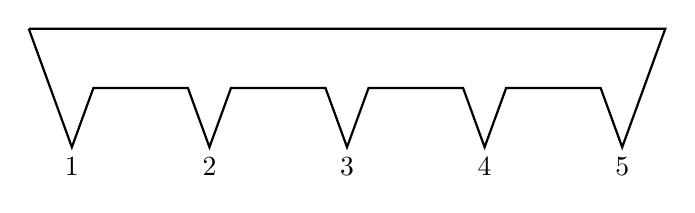
\begin{tikzpicture}[scale=.8]
\coordinate (O) at (0,0);
\draw [thick] (O) -- (++110:1cm) coordinate (P);
\draw[thick] (O) --
  ++(-70:1cm) coordinate(A) node[below] {$1$} -- 
  ++(+70:1cm) -- ++(0:1.5cm) --
  ++(-70:1cm) coordinate(B) node[below] {$2$} -- 
  ++(+70:1cm) -- ++(0:1.5cm) --
  ++(-70:1cm) coordinate(C) node[below] {$3$}-- 
  ++(+70:1cm) -- ++(0:1.5cm) --
  ++(-70:1cm) coordinate(D) node[below] {$4$} -- 
  ++(+70:1cm) -- ++(0:1.5cm) --
  ++(-70:1cm) coordinate(E) node[below] {$5$} --
  ++(+70:2cm) -- (P);

\end{tikzpicture}
\end{center}
\caption{Un museo cuyas paredes no forman un polígono convexo}\label{f.museum.nonconvex}
\end{figure}

\begin{figure}[t]
\begin{center}
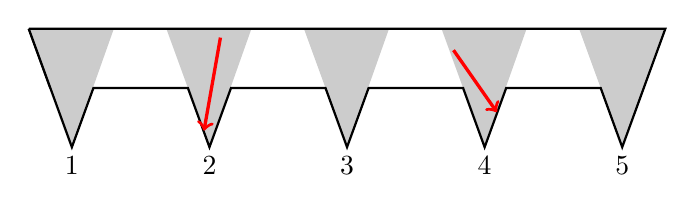
\begin{tikzpicture}[scale=.8]
\coordinate (O) at (0,0);
\draw [thick] (O) -- (++110:1cm) coordinate (P);
\path (O) --
  ++(-70:1cm) coordinate(A) node[below] {$1$} -- 
  ++(+70:1cm) coordinate(A1) -- ++(0:1.5cm) coordinate(A2) --
  ++(-70:1cm) coordinate(B) node[below] {$2$} -- 
  ++(+70:1cm) coordinate(B1) -- ++(0:1.5cm) coordinate(B2) --
  ++(-70:1cm) coordinate(C) node[below] {$3$}-- 
  ++(+70:1cm) coordinate(C1) -- ++(0:1.5cm) coordinate(C2) --
  ++(-70:1cm) coordinate(D) node[below] {$4$} -- 
  ++(+70:1cm) coordinate(D1) -- ++(0:1.5cm) coordinate(D2) --
  ++(-70:1cm) coordinate(E) node[below] {$5$} --
  ++(+70:2cm) coordinate(E1) -- (P);

\path[fill,black!20!white] (A) -- ++(110:2cm) -- ++(0:1.35cm)-- cycle;
\path[fill,black!20!white] (B) -- ++(110:2cm) -- ++(0:1.35cm)-- cycle;
\path[fill,black!20!white] (C) -- ++(110:2cm) -- ++(0:1.35cm)-- cycle;
\path[fill,black!20!white] (D) -- ++(110:2cm) -- ++(0:1.35cm)-- cycle;
\path[fill,black!20!white] (E) -- ++(110:2cm) -- ++(0:1.35cm)-- cycle;

\draw[thick] (P) -- (O) -- (A) -- (A1) -- (A2) --
   (B) -- (B1) -- (B2) -- (C) -- (C1) -- (C2) --
   (D) -- (D1) -- (D2) -- (E) -- (E1) -- (P);

\coordinate (G1) at (2.7,.8);
\coordinate (G2) at (6.4,.6);
\draw[->,red,very thick] (G1) -- +(-100:1.5cm);
\draw[->,red,very thick] (G2) -- +(-55:1.2cm);
\vertexcolor{G1}{red};
\vertexcolor{G2}{red};
\end{tikzpicture}
\end{center}
\caption{Visibilidad dentro de cada ``diente''}\label{f.visibility-tooth}
\end{figure}

Si al menos uno de los guardias se coloca cerca de la pared superior que abarca todo el museo, podrá observar todas las paredes horizontales (flechas azules en la Fig.~\ref{f.museum.shaded}). Así pues, bastan $5=15/3$ guardias para observar todas las paredes del museo. Como los triángulos no se superponen, un vigilante de un triángulo no podrá observar todas las paredes de otro triángulo (flecha verde), por lo que se necesitan $5$ vigilantes.

\begin{figure}[ht]
\begin{center}
\begin{tikzpicture}[scale=.8]
\coordinate (O) at (0,0);
\draw [thick] (O) -- (++110:1cm) coordinate (P);
\path (O) --
  ++(-70:1cm) coordinate(A) node[below] {$1$} -- 
  ++(+70:1cm) coordinate(A1) -- ++(0:1.5cm) coordinate(A2) --
  ++(-70:1cm) coordinate(B) node[below] {$2$} -- 
  ++(+70:1cm) coordinate(B1) -- ++(0:1.5cm) coordinate(B2) --
  ++(-70:1cm) coordinate(C) node[below] {$3$}-- 
  ++(+70:1cm) coordinate(C1) -- ++(0:1.5cm) coordinate(C2) --
  ++(-70:1cm) coordinate(D) node[below] {$4$} -- 
  ++(+70:1cm) coordinate(D1) -- ++(0:1.5cm) coordinate(D2) --
  ++(-70:1cm) coordinate(E) node[below] {$5$} --
  ++(+70:2cm) coordinate(E1) -- (P);

\path[fill,black!20!white] (A) -- ++(110:2cm) -- ++(0:1.35cm)-- cycle;
\path[fill,black!20!white] (B) -- ++(110:2cm) -- ++(0:1.35cm)-- cycle;
\path[fill,black!20!white] (C) -- ++(110:2cm) -- ++(0:1.35cm)-- cycle;
\path[fill,black!20!white] (D) -- ++(110:2cm) -- ++(0:1.35cm)-- cycle;
\path[fill,black!20!white] (E) -- ++(110:2cm) -- ++(0:1.35cm)-- cycle;

\draw[thick] (P) -- (O) -- (A) -- (A1) -- (A2) --
   (B) -- (B1) -- (B2) -- (C) -- (C1) -- (C2) --
   (D) -- (D1) -- (D2) -- (E) -- (E1) -- (P);

\coordinate (G1) at (9,.8);
\coordinate (G2) at ($(O)+(.5,.5)$);
\draw[->,very thick,green!80!black,dashed] (G1) -- +(-165:4.6cm);
\draw[->,very thick,blue] (G2) -- ++(7.4,.35);
\draw[->,very thick,blue] (G2) -- ++(2.9,-.42);
\draw[thick] (6,0) circle(4pt);
\draw[thick] (4.95,-.28) circle(4pt);
\vertexcolor{G1}{green!80!black};
\vertexcolor{G2}{blue};
\end{tikzpicture}
\end{center}
\caption{Visibilidad de las paredes del museo}\label{f.museum.shaded}
\end{figure}

El ejemplo de la Fig.~\ref{f.museum.nonconvex} puede generalizarse a $n/3$ dientes con $n$ paredes, por lo que concluimos que \emph{al menos} $n/3$ guardas son necesarios. Queremos demostrar que $n/3$ guardianes son suficientes para vigilar cualquier museo.

La sección~\ref{s.museum-triangulating} demuestra que cualquier polígono triangulado puede ser tricolor. Esto se utiliza en la sección~\ref{s.museum-guard} para demostrar el teorema de que $n/3$ guardias son suficientes. La sección~\ref{s.museum-triangulated} completa la demostración demostrando que cualquier polígono puede ser triangulado.

\section{Colorear polígonos triangulados}\label{s.museum-triangulating}

\begin{definition}
Una \emph{diagonal} a de un polígono es una segmento que une dos vértices y que no es una de los lados del polígono.
\end{definition}

\begin{definition}
Un polígono puede ser \emph{triangulado} si se pueden construir diagonales no intersecantes de manera que el interior del polígono esté cubierto por triángulos.
\end{definition}\index{Polygon!triangulated}

\begin{theorem}
Cualquier polígono puede triangularse.\label{thm.tri}
\end{theorem}
Aplazamos la demostración de este Teorema.
\begin{definition}
Un vértice de un polígono es \emph{convexo}\index{Polígono!vértices convexos y cóncavos} si su ángulo interior es menor que $180^\circ$; un vértice es \emph{cóncavo} si su ángulo interior es mayor que $180^\circ$. 
\end{definition}
En la Fig.~\ref{f.museum.arbitrary} el vértice $1$ es convexo y el vértice $2$ es cóncavo.

\begin{figure}[ht]
\begin{center}
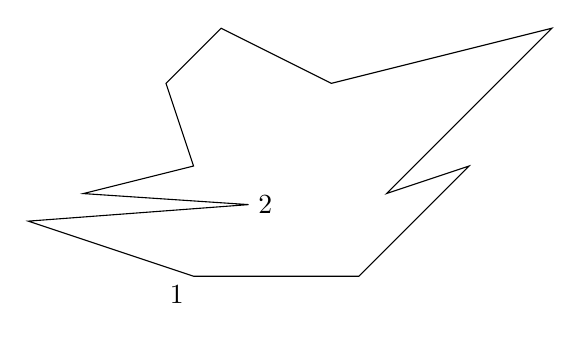
\begin{tikzpicture}[scale=.7]
\draw
  (0,0) coordinate (A) node[below left] {$1$} -- 
  ++(3,0) coordinate (B) --
  ++(2,2) coordinate (C) --
  ++(-1.5,-.5) coordinate (D) --
  ++(3,3) coordinate (E) -- 
  ++(-4,-1) coordinate (F) --
  ++(-2,1) coordinate (G) --
  ++(-1,-1) coordinate (H) --
  ++(.5,-1.5) coordinate (I) --
  ++(-2,-.5) coordinate (J) --
  ++(3,-.2) coordinate (K) node[right] {$2$} -- 
  ++(-4,-.3) coordinate (L) --
  cycle;
\vertex{A};
\vertex{K};
\end{tikzpicture}
\end{center}
\caption{Un polígono con un vértice convexo ($1$) y un vértice cóncavo ($2$)}\label{f.museum.arbitrary}
\end{figure}

\begin{definition}
Un polígono con vértices $V$ puede ser \emph{coloreado con tres colores} si existe una correspondencia:
\[c: V \mapsto \{\mathit{red},\mathit{blue},\mathit{green}\}\,,\]
tal que ningun lado tenga dos vértices con el mismo color.
\end{definition}

\begin{theorem}
Un polígono triangulado puede ser coloreado con tres colores.\label{thm.colored}
\end{theorem}\index{Coloring!polygon@of a polygon}

\begin{proof}
Por inducción sobre el número de vértices. Un triángulo puede ser coloreado con tres colores. Un polígono triangulado con $n>3$ vértices debe tener una diagonal. Elegimos una diagonal arbitraria $\overline{AB}$ (Fig.~\ref{f.museum.three-1}) y dividimos el polígono a lo largo de esta diagonal en dos polígonos más pequeños (Fig.~\ref{f.museum.three-2}). Por inducción, cada uno de estos polígonos más pequeños puede ser de tres colores (Fig.~\ref{f.museum.three-3}).

Como los colores asignados son arbitrarios, si se asignan colores diferentes a $A,B$ en los dos polígonos, podemos reasignar los colores en uno de ellos para que los colores de $A,B$ sean los mismos en ambos polígonos. Por ejemplo, en la Fig.~\ref{f.museum.three-4} intercambiamos \emph{rojo} y \emph{verde} en el polígono inferior.
Adosamos los dos polígonos para recuperar el polígono original con $ n $ vértices. Este será de tres colores (Fig.~\ref{f.museum.three-5}).
\end{proof}

\begin{figure}[t]
\begin{minipage}{.45\textwidth}
\begin{center}
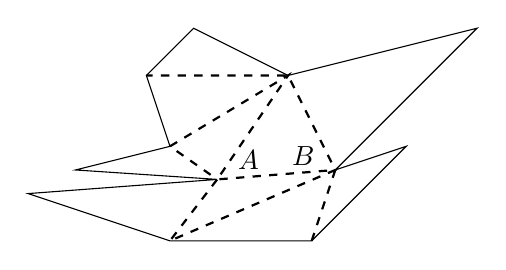
\begin{tikzpicture}[scale=.6]
\draw
  (0,0) coordinate (A) -- 
  ++(3,0) coordinate (B) --
  ++(2,2) coordinate (C) --
  ++(-1.5,-.5) coordinate (D) --
  ++(3,3) coordinate (E) -- 
  ++(-4,-1) coordinate (F) --
  ++(-2,1) coordinate (G) --
  ++(-1,-1) coordinate (H) --
  ++(.5,-1.5) coordinate (I) --
  ++(-2,-.5) coordinate (J) --
  ++(3,-.2) coordinate (K) -- 
  ++(-4,-.3) coordinate (L) --
  cycle;
\vertex{K};
\vertex{D};
\node[above right,xshift=4pt] at (K) {$A$};
\node[above left,xshift=-4pt,yshift=-2pt] at (D) {$B$};

\draw[thick,dashed]
  (B) -- (D) -- (K) -- (F) -- (I) -- (K) -- (A) -- (D) -- (F) -- (H);
\end{tikzpicture}
\caption{Una diagonal arbitraria en un polígono}\label{f.museum.three-1}
\end{center}
\end{minipage}
\hfill
\begin{minipage}{.45\textwidth}
\begin{center}
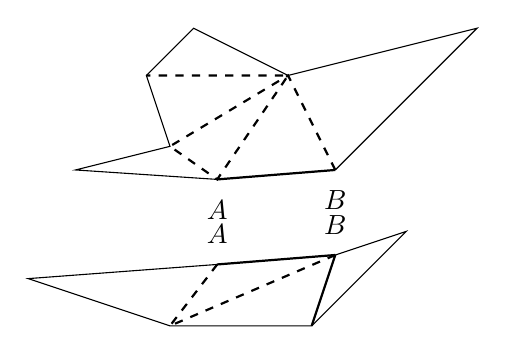
\begin{tikzpicture}[scale=.6]
\path
  (0,0) coordinate (A1) -- 
  ++(3,0) coordinate (B1) --
  ++(2,2) coordinate (C1) --
  ++(-1.5,-.5) coordinate (D1);
\draw
  (D1) --
  ++(3,3) coordinate (E1) -- 
  ++(-4,-1) coordinate (F1) --
  ++(-2,1) coordinate (G1) --
  ++(-1,-1) coordinate (H1) --
  ++(.5,-1.5) coordinate (I1) --
  ++(-2,-.5) coordinate (J1) --
  ++(3,-.2) coordinate (K1);
\path
  (K1) -- 
  ++(-4,-.3) coordinate (L1) --
  (A1);
\vertex{K1};
\vertex{D1};
\node[below,yshift=-4pt] at (K1) {$A$};
\node[below,yshift=-4pt] at (D1) {$B$};

\draw[thick,dashed]
  (D1) -- (F1) -- (I1) -- (K1) -- (F1) -- (H1);
\draw[thick] (D1) -- (K1);

\begin{scope}[yshift=-1.8cm]
\draw
  (0,0) coordinate (A2) -- 
  ++(3,0) coordinate (B2) --
  ++(2,2) coordinate (C2) --
  ++(-1.5,-.5) coordinate (D2);
\path
  (D2) --
  ++(3,3) coordinate (E2) --
  ++(-4,-1) coordinate (F2) --
  ++(-2,1) coordinate (G2) --
  ++(-1,-1) coordinate (H2) --
  ++(.5,-1.5) coordinate (I2) --
  ++(-2,-.5) coordinate (J2) --
  ++(3,-.2) coordinate (K2);
\draw
  (K2) --
  ++(-4,-.3) coordinate (L2) --
  (A2);
\vertex{K2};
\vertex{D2}; 
\node[above,yshift=4pt] at (K2) {$A$};
\node[above,yshift=4pt] at (D2) {$B$};

\draw[thick,dashed]
  (K2) -- (A2) -- (D2) -- (B2) -- (D2);
\draw[thick] (D2) -- (K2);
\end{scope}
\end{tikzpicture}
\caption{División del polígono}\label{f.museum.three-2}
\end{center}
\end{minipage}
\end{figure}

\begin{figure}[t]
\begin{minipage}{.45\textwidth}
\begin{center}
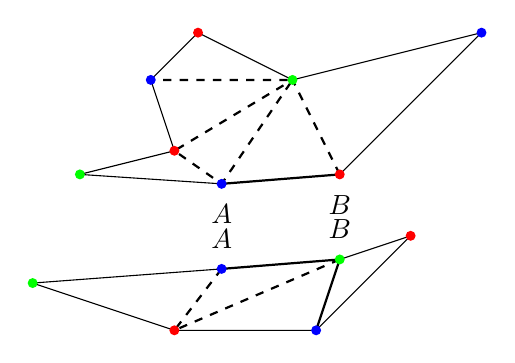
\begin{tikzpicture}[scale=.6]
\path
  (0,0) coordinate (A1) -- 
  ++(3,0) coordinate (B1) --
  ++(2,2) coordinate (C1) --
  ++(-1.5,-.5) coordinate (D1);
\draw
  (D1) --
  ++(3,3) coordinate (E1) -- 
  ++(-4,-1) coordinate (F1) --
  ++(-2,1) coordinate (G1) --
  ++(-1,-1) coordinate (H1) --
  ++(.5,-1.5) coordinate (I1) --
  ++(-2,-.5) coordinate (J1) --
  ++(3,-.2) coordinate (K1);
\path
  (K1) -- 
  ++(-4,-.3) coordinate (L1) --
  (A1);
  
\draw[thick,dashed]
  (D1) -- (F1) -- (I1) -- (K1) -- (F1) -- (H1);
\draw[thick] (D1) -- (K1);

\node[below,yshift=-4pt] at (K1) {$A$};
\node[below,yshift=-4pt] at (D1) {$B$};

\foreach \point/\color in {D1/red,E1/blue,F1/green,G1/red,H1/blue,I1/red,J1/green,K1/blue}
  \fill[color=\color] (\point) circle(3pt);

\begin{scope}[yshift=-1.8cm]

\draw
  (0,0) coordinate (A2) -- 
  ++(3,0) coordinate (B2) --
  ++(2,2) coordinate (C2) --
  ++(-1.5,-.5) coordinate (D2);
\path
  (D2) --
  ++(3,3) coordinate (E2) --
  ++(-4,-1) coordinate (F2) --
  ++(-2,1) coordinate (G2) --
  ++(-1,-1) coordinate (H2) --
  ++(.5,-1.5) coordinate (I2) --
  ++(-2,-.5) coordinate (J2) --
  ++(3,-.2) coordinate (K2);
\draw
  (K2) --
  ++(-4,-.3) coordinate (L2) --
  (A2);
  
\draw[thick,dashed]
  (K2) -- (A2) -- (D2) -- (B2) -- (D2);
\draw[thick] (D2) -- (K2);
\node[above,yshift=4pt] at (K2) {$A$};
\node[above,yshift=4pt] at (D2) {$B$};

\foreach \point/\color in {A2/red,B2/blue,C2/red,D2/green,K2/blue,L2/green}
  \fill[color=\color] (\point) circle(3pt);

\end{scope}
\end{tikzpicture}
\caption{Coloración con tres colores de los dos polígonos más pequeños}\label{f.museum.three-3}
\end{center}
\end{minipage}
\hfill
\begin{minipage}{.45\textwidth}
\begin{center}
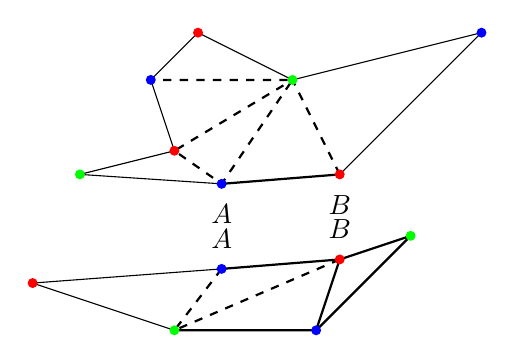
\begin{tikzpicture}[scale=.6]
\path
  (0,0) coordinate (A1) -- 
  ++(3,0) coordinate (B1) --
  ++(2,2) coordinate (C1) --
  ++(-1.5,-.5) coordinate (D1);
\draw
  (D1) --
  ++(3,3) coordinate (E1) -- 
  ++(-4,-1) coordinate (F1) --
  ++(-2,1) coordinate (G1) --
  ++(-1,-1) coordinate (H1) --
  ++(.5,-1.5) coordinate (I1) --
  ++(-2,-.5) coordinate (J1) --
  ++(3,-.2) coordinate (K1);
\path
  (K1) -- 
  ++(-4,-.3) coordinate (L1) --
  (A1);
  
\node[below,yshift=-4pt] at (K1) {$A$};
\node[below,yshift=-4pt] at (D1) {$B$};

\draw[thick,dashed]
  (D1) -- (F1) -- (I1) -- (K1) -- (F1) -- (H1);
\draw[thick] (D1) -- (K1);

\foreach \point/\color in {D1/red,E1/blue,F1/green,G1/red,H1/blue,I1/red,J1/green,K1/blue}
  \fill[color=\color] (\point) circle(3pt);

\begin{scope}[yshift=-1.8cm]

\draw[thick]
  (0,0) coordinate (A2) -- 
  ++(3,0) coordinate (B2) --
  ++(2,2) coordinate (C2) --
  ++(-1.5,-.5) coordinate (D2);
\path
  (D2) --
  ++(3,3) coordinate (E2) --
  ++(-4,-1) coordinate (F2) --
  ++(-2,1) coordinate (G2) --
  ++(-1,-1) coordinate (H2) --
  ++(.5,-1.5) coordinate (I2) --
  ++(-2,-.5) coordinate (J2) --
  ++(3,-.2) coordinate (K2);
\draw
  (K2) --
  ++(-4,-.3) coordinate (L2) --
  (A2);
  
\draw[thick,dashed]
  (K2) -- (A2) -- (D2) -- (B2) -- (D2);
\draw[thick] (D2) -- (K2);
\node[above,yshift=4pt] at (K2) {$A$};
\node[above,yshift=4pt] at (D2) {$B$};

\foreach \point/\color in {A2/green,B2/blue,C2/green,D2/red,K2/blue,L2/red}
  \fill[color=\color] (\point) circle(3pt);

\end{scope}
\end{tikzpicture}
\caption{Cambio de los colores de un polígono para que coincidan con los del otro}\label{f.museum.three-4}
\end{center}
\end{minipage}
\end{figure}

\begin{figure}[t]
\begin{center}
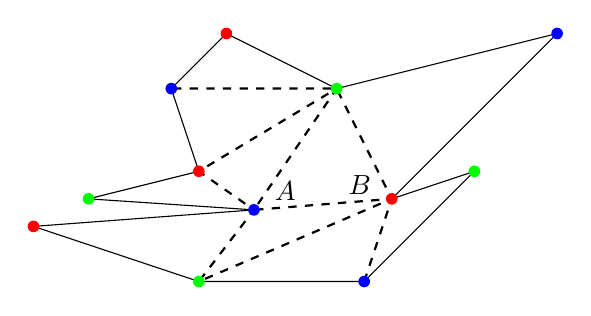
\begin{tikzpicture}[scale=.7]
\draw
  (0,0) coordinate (A) -- 
  ++(3,0) coordinate (B) --
  ++(2,2) coordinate (C) --
  ++(-1.5,-.5) coordinate (D) --
  ++(3,3) coordinate (E) -- 
  ++(-4,-1) coordinate (F) --
  ++(-2,1) coordinate (G) --
  ++(-1,-1) coordinate (H) --
  ++(.5,-1.5) coordinate (I) --
  ++(-2,-.5) coordinate (J) --
  ++(3,-.2) coordinate (K) -- 
  ++(-4,-.3) coordinate (L) --
  cycle;
  
\node[above right,xshift=4pt] at (K) {$A$};
\node[above left,xshift=-4pt,yshift=-2pt] at (D) {$B$};

\draw[thick,dashed]
  (B) -- (D) -- (K) -- (F) -- (I) -- (K) -- (A) -- (D) -- (F) -- (H);

\foreach \point/\color in {D/red,E/blue,F/green,G/red,H/blue,I/red,J/green,K/blue,A/green,B/blue,C/green,L/red}
  \fill[color=\color] (\point) circle(3pt);

\end{tikzpicture}
\end{center}
\caption{Vuelve a pegar los dos polígonos más pequeños}\label{f.museum.three-5}
\end{figure}

\section{De colorear polígonos a vigilar un museo}\label{s.museum-guard}

\begin{theorem}\label{thm.guarded}
Un museo con $n$ paredes puede estar vigilado por $n/3$ guardias.
\end{theorem}\index{Museum!triangulated@and triangulated polygons}
\begin{proof}
Por el Teorema~\ref{thm.tri} el polígono puede ser triangulado y por el Teorema~\ref{thm.colored} el polígono puede ser coloreado con tres colores. Los tres vértices de cada triángulo en la triangulación deben ser coloreados por colores diferentes con el fin de satisfacer la condición de ser de tres colores. Dado que el polígono es de tres colores, al menos un color, por ejemplo rojo, puede aparecer como máximo $n/3$ veces, y cada triángulo debe tener un vértice de color rojo. Coloquemos un guardia en cada vértice rojo; o ella puede observar todas las paredes de los triángulos a los que pertenece el vértice. Como los triángulos de la triangulación incluyen todos los lados del polígono, $n/3$ guardias son suficientes para vigilar todas las paredes del museo.
\end{proof}
Si $n$ no es divisible por $3$ el número de vigilantes necesarios es $\lfloor n/3\rfloor$, el mayor número entero menor o igual que $n/3$. Por ejemplo, $4$ guardias son suficientes para museos con paredes de $12, 13, 14$ ya que $\lfloor 12/3\rfloor =\lfloor 13/3\rfloor=\lfloor 14/3\rfloor=4$. Para simplificar, ignoramos esta complicación.
 
\section{Cualquier polígono puede triangularse}\label{s.museum-triangulated}

\begin{theorem}\label{thm.interior-angles-of-a-polygon}
La suma de los ángulos interiores de un polígono con $n$ vértices es:
\[180^\circ(n-2)\,.\]
\end{theorem}\index{Polygon!triangulated}
\begin{proof}
Consideremos un polígono convexo y denotemos su \emph{ángulos exteriores} por $\theta_i$ (Fig.~\ref{f.museum.exterior}).
Al pasar de una línea discontinua a la siguiente, se completa una rotación alrededor de un círculo así:
\[
\sum_{i=1}^n \theta_i = 360^\circ\,.
\]
\begin{figure}[t]
\begin{center}
\begin{tikzpicture}[scale=.5]
\coordinate (O) at (0,0);
\foreach \x/\name/\n/\po in {0/a/A/right,.6/b/B/above,1.6/c/C/left,2.4/d/D/below left,3.9/e/E/below right} {
  \coordinate (\name) at ($(O)+(\x*72+18:3cm)$);
}
\draw[thick] (a) -- (b) -- (c) -- (d) --(e) -- cycle;

\draw[thick,dashed] (a) 
  node[above,xshift=-2pt,yshift=8pt] {$\theta_1$} -- 
  ($(a)!2!(b)$);
\draw[thick,dashed] (b)
  node[above left,xshift=-8pt,yshift=0pt] {$\theta_2$} -- 
  ($(b)!1.7!(c)$);
\draw[thick,dashed] (c) 
  node[below left,xshift=-4pt,yshift=-2pt] {$\theta_3$} -- 
  ($(c)!1.7!(d)$);
\draw[thick,dashed] (d)
  node[below right,xshift=0pt,yshift=-4pt] {$\theta_4$} -- 
  ($(d)!1.5!(e)$);
\draw[thick,dashed] (e)
  node[right,xshift=4pt,yshift=4pt] {$\theta_5$} -- 
  ($(e)!1.7!(a)$);

\end{tikzpicture}
\end{center}
\caption{Los ángulos exteriores de un polígono convexo}\label{f.museum.exterior}
\end{figure}
Para cada ángulo exterior $\theta_i$ denotemos su correspondiente ángulo interior por $\phi_i$. Entonces:
\begin{eqnarray*}
\displaystyle\sum_{i=1}^n \theta_i &=&\displaystyle\sum_{i=1}^n (180^\circ-\phi_i)= 360^\circ\\
\displaystyle\sum_{i=1}^n \phi_i &=& n\cdot 180^\circ-360^\circ =180^\circ(n-2)\,.
\end{eqnarray*}
Si existe un vértice cóncavo ($B$ en la Fig.~\ref{f.museum.concave}), existe un triángulo formado por los dos lados incidentes con el vértice cóncavo y la recta $\overline{AC}$ que une los otros dos vértices. Sumando los ángulos del triángulo obtenemos:
\begin{eqnarray*}
(180^\circ - \alpha) + (360^\circ - \beta) + (180^\circ - \gamma) &=& 180^\circ\\
\alpha + \beta + \gamma &=& 3\cdot 180^\circ\,.
\end{eqnarray*}

La suma de los ángulos interiores aumenta en $\alpha+\beta+\gamma$ mientras que el número de vértices aumenta en tres conservando la ecuación del teorema:
\begin{eqnarray*}
\displaystyle\sum_{i=1}^n \phi_i + (\alpha + \beta + \gamma) &=& 180^\circ(n-2)+3\cdot 180^\circ\\
&=& 180^\circ((n+3)-2)\,.
\end{eqnarray*}
\end{proof}

\begin{figure}[t]
\begin{center}
\begin{tikzpicture}[scale=.8]
\draw[thick] (0,0) -- 
  (3,0) coordinate (A) node[above left,yshift=8pt] {$\alpha$} --
  ++(60:2) coordinate (B) node[above,yshift=8pt] {$\beta$} --
  ++(-60:2) coordinate (C) 
    node[above right,yshift=8pt] {$\gamma$}  --
  ++(3,0);

\draw ($(A)+(-.4,0)$) arc(180:60:.4);
\draw ($(B)+(-60:.3)$) arc(-60:240:.3);
\draw ($(C)+(.4,0)$) arc(0:120:.4);
\node[below] at (A) {$A$};
\node[below,yshift=-5pt] at (B) {$B$};
\node[below] at (C) {$C$};
\draw[thick,dashed] (A) -- (C);
\end{tikzpicture}
\end{center}
\caption{Un vértice cóncavo}\label{f.museum.concave}
\end{figure}

\begin{theorem}\label{thm.convex}
En un polígono debe haber al menos tres vértices convexos.
\end{theorem}

\begin{proof}
Sea $k$ el número de vértices cóncavos donde el ángulo interior de cada uno es $180^\circ+\epsilon_i$, $\epsilon_i>0$. La suma de los ángulos interiores de los vértices cóncavos es ciertamente menor o igual que la suma de los ángulos interiores de todos los vértices:
\begin{eqnarray*}
k\cdot 180^\circ +\displaystyle\sum_{i=1}^{k}\epsilon_i &\leq& 180^\circ(n-2)\\
(k+2)\cdot 180^\circ +\displaystyle\sum_{i=1}^{k}\epsilon_i &\leq& n\cdot 180^\circ\\
(k+2)\cdot 180^\circ &<& n\cdot 180^\circ\\
k&<&n-2\,.
\end{eqnarray*}
De ello se deduce que debe haber al menos tres vértices que sean convexos, no cóncavos.
\end{proof}

\noindent{}Ahora podemos demostrar el Teorema~\ref{thm.tri}.

\begin{proof}
Por inducción en el número de vértices. Para $n=3$ no hay nada que demostrar. Si $n>3$, por el Teorema~\ref{thm.convex} debe haber un vértice $C$ convexo. Denotamos sus vértices adyacentes por $B,D$. Si $\overline{BD}$ está contenida en el polígono (Fig.~\ref{f.contained}), es una diagonal y el polígono se puede dividir en $\triangle BCD$ y otro polígono $\overline{ABDE}$ con $\overline{BD}$ como lado y que es más pequeño que el polígono original (Fig.~\ref{f.contained}). Por la hipótesis inductiva, el polígono se puede triangular y luego adosar de nuevo a $\triangle BCD$, triangulando el polígono original.

\begin{figure}[t]
\begin{minipage}{.45\textwidth}
\begin{center}
\begin{tikzpicture}[scale=1.4]
\clip (-.5,-.4) rectangle (3.8,2.2);
\draw
  (0,0) coordinate (A) -- 
  ++(1.5,0) coordinate (B) --
  ++(2,2) coordinate (C) --
  ++(-1.8,-.5) coordinate (D) --
  ++(-1,.5) coordinate (E) --
  (A);
\draw[thick,dashed] (B) -- (D);
\foreach \point/\pos in {A/below,B/below,C/right,D/above,E/left}
  \node[\pos] at (\point) {$\point$};
\vertex{B};
\vertex{D};
\end{tikzpicture}
\caption{Triangulación en la que una diagonal está contenida en el polígono}\label{f.contained}
\end{center}
\end{minipage}
\hfill
\begin{minipage}{.45\textwidth}
\begin{center}
\begin{tikzpicture}[scale=1.4]
\clip (-.2,-.4) rectangle (3.8,2.2);
\draw
  (0,0) coordinate (A) -- 
  ++(1.5,0) coordinate (B) --
  ++(2,2) coordinate (C) --
  ++(-1.8,-.5) coordinate (D) --
  ++(-1,.5) coordinate (E) --
  ++(1.3,-1) coordinate (F) --
  (A);
\draw[thick,dashed] (B) -- (D);
\draw[very thick,dotted] (C) -- (F);
\node [draw,circle through=(F)] at (C) {};
\node[below] at (A) {$A$};
\node[below] at (B) {$B$};
\node[right] at (C) {$C$};
\node[above,yshift=2pt,xshift=-3pt] at (D) {$D$};
\node[left]  at (E) {$E$};
\node[below,yshift=-1pt,xshift=-2pt] at (F) {$F$};
\vertex{C};
\vertex{F};
\end{tikzpicture}
\caption{Triangulación en la que una diagonal no está contenida en el polígono}\label{f.museum.concave-vertices}
\end{center}
\end{minipage}
\end{figure}

Si $\overline{BD}$ no está contenido en el polígono, debe haber un vértice cóncavo $F$ que es \emph{más cercano} a $C$ (Fig.~\ref{f.museum.concave-vertices}). $\overline{CF}$ es una diagonal y divide el polígono en dos polígonos más pequeños $\overline{CFED}$ y $\overline{CFAB}$. Por la hipótesis inductiva estos pueden ser triangulados y adosadas.
\end{proof}

\subsection*{¿Cuál es la sorpresa?}
El teorema del museo es sorprendente porque lo que parece un teorema de geometría se demuestra con bastante elegancia apelando a la coloración de un grafo.

\subsection*{Fuentes}

Este capítulo está basado en \cite[Capítulo~39]{thebook}.
